%%%%%%%%%%%%%%%%%%%%%%%%%%%%%%%%%%%%%%%%%
% Bloom filter
% Module dist
% Assignment 02
%
% This template was downloaded from:
% http://www.LaTeXTemplates.com
%
% Authors:
% Marco Romanutti
% Dominik Fringeli
%
% License:
% CC BY-NC-SA 3.0 (http://creativecommons.org/licenses/by-nc-sa/3.0/)
%
%%%%%%%%%%%%%%%%%%%%%%%%%%%%%%%%%%%%%%%%%

%----------------------------------------------------------------------------------------
%	PACKAGES AND OTHER DOCUMENT CONFIGURATIONS
%----------------------------------------------------------------------------------------

\documentclass[10pt, a4paper, twocolumn]{article} % 10pt font size (11 and 12 also possible), A4 paper (letterpaper for US letter) and two column layout (remove for one column)

%%%%%%%%%%%%%%%%%%%%%%%%%%%%%%%%%%%%%%%%%
% Bloom filter
% Module dist
% Assignment 02
%
% This template was downloaded from:
% http://www.LaTeXTemplates.com
%
% Authors:
% Marco Romanutti
% Dominik Fringeli
%
% License:
% CC BY-NC-SA 3.0 (http://creativecommons.org/licenses/by-nc-sa/3.0/)
%
%%%%%%%%%%%%%%%%%%%%%%%%%%%%%%%%%%%%%%%%%

%----------------------------------------------------------------------------------------
%	PACKAGES AND OTHER DOCUMENT CONFIGURATIONS
%----------------------------------------------------------------------------------------

\usepackage[english]{babel} % English language hyphenation

\usepackage{microtype} % Better typography

\usepackage{amsmath,amsfonts,amsthm} % Math packages for equations

\usepackage[svgnames]{xcolor} % Enabling colors by their 'svgnames'

\usepackage[hang, small, labelfont=bf, up, textfont=it]{caption} % Custom captions under/above tables and figures

\usepackage{booktabs} % Horizontal rules in tables

\usepackage{lastpage} % Used to determine the number of pages in the document (for "Page X of Total")

\usepackage{graphicx} % Required for adding images
\usepackage{float} % Force image placement

\usepackage{enumitem} % Required for customising lists
\setlist{noitemsep} % Remove spacing between bullet/numbered list elements

\usepackage{sectsty} % Enables custom section titles

\usepackage{tabularx} % Pro/cons table
\allsectionsfont{\usefont{OT1}{phv}{b}{n}} % Change the font of all section commands (Helvetica)

%----------------------------------------------------------------------------------------
%	MARGINS AND SPACING
%----------------------------------------------------------------------------------------

\usepackage{geometry} % Required for adjusting page dimensions

\geometry{
	top=1cm, % Top margin
	bottom=1.5cm, % Bottom margin
	left=2cm, % Left margin
	right=2cm, % Right margin
	includehead, % Include space for a header
	includefoot, % Include space for a footer
	%showframe, % Uncomment to show how the type block is set on the page
}

\setlength{\columnsep}{7mm} % Column separation width

%----------------------------------------------------------------------------------------
%	FONTS
%----------------------------------------------------------------------------------------

\usepackage[T1]{fontenc} % Output font encoding for international characters
\usepackage[utf8]{inputenc} % Required for inputting international characters

\usepackage{XCharter} % Use the XCharter font

%----------------------------------------------------------------------------------------
%	HEADERS AND FOOTERS
%----------------------------------------------------------------------------------------

\usepackage{fancyhdr} % Needed to define custom headers/footers
\pagestyle{fancy} % Enables the custom headers/footers

\renewcommand{\headrulewidth}{0.0pt} % No header rule
\renewcommand{\footrulewidth}{0.4pt} % Thin footer rule

\renewcommand{\sectionmark}[1]{\markboth{#1}{}} % Removes the section number from the header when \leftmark is used

%\nouppercase\leftmark % Add this to one of the lines below if you want a section title in the header/footer

% Headers
\lhead{} % Left header
\chead{\textit{\thetitle}} % Center header - currently printing the article title
\rhead{} % Right header

% Footers
\lfoot{} % Left footer
\cfoot{} % Center footer
\rfoot{\footnotesize Seite \thepage\ von \pageref{LastPage}} % Right footer, "Page 1 of 2"

\fancypagestyle{firstpage}{ % Page style for the first page with the title
	\fancyhf{}
	\renewcommand{\footrulewidth}{0pt} % Suppress footer rule
}

%----------------------------------------------------------------------------------------
%	TITLE SECTION
%----------------------------------------------------------------------------------------

\newcommand{\authorstyle}[1]{{\large\usefont{OT1}{phv}{b}{n}\color{DarkRed}#1}} % Authors style (Helvetica)

\newcommand{\institution}[1]{{\footnotesize\usefont{OT1}{phv}{m}{sl}\color{Black}#1}} % Institutions style (Helvetica)

\usepackage{titling} % Allows custom title configuration

\newcommand{\HorRule}{\color{DarkGoldenrod}\rule{\linewidth}{1pt}} % Defines the gold horizontal rule around the title

\pretitle{
	\vspace{0pt} % Move the entire title section up
	\HorRule\vspace{10pt} % Horizontal rule before the title
	\fontsize{32}{36}\usefont{OT1}{phv}{b}{n}\selectfont % Helvetica
	\color{DarkRed} % Text colour for the title and author(s)
}

\posttitle{\par\vskip 15pt} % Whitespace under the title

\preauthor{} % Anything that will appear before \author is printed

\postauthor{ % Anything that will appear after \author is printed
	\vspace{10pt} % Space before the rule
	\par\HorRule % Horizontal rule after the title
	\vspace{-34pt} % Space after the title section
}

%----------------------------------------------------------------------------------------
%	ABSTRACT
%----------------------------------------------------------------------------------------

\usepackage{lettrine} % Package to accentuate the first letter of the text (lettrine)
\usepackage{fix-cm}	% Fixes the height of the lettrine

\newcommand{\initial}[1]{ % Defines the command and style for the lettrine
	\lettrine[lines=3,findent=4pt,nindent=0pt]{% Lettrine takes up 3 lines, the text to the right of it is indented 4pt and further indenting of lines 2+ is stopped
		\color{DarkGoldenrod}% Lettrine colour
		{#1}% The letter
	}{}%
}

\usepackage{xstring} % Required for string manipulation

\newcommand{\lettrineabstract}[1]{
	\StrLeft{#1}{1}[\firstletter] % Capture the first letter of the abstract for the lettrine
	\initial{\firstletter}\textbf{\StrGobbleLeft{#1}{1}} % Print the abstract with the first letter as a lettrine and the rest in bold
}

%----------------------------------------------------------------------------------------
%	BIBLIOGRAPHY
%----------------------------------------------------------------------------------------

\usepackage[backend=bibtex,style=authoryear,natbib=true]{biblatex} % Use the bibtex backend with the authoryear citation style (which resembles APA)

\addbibresource{example.bib} % The filename of the bibliography

\usepackage[autostyle=true]{csquotes} % Required to generate language-dependent quotes in the bibliography
 % Specifies the document structure and loads requires packages

%----------------------------------------------------------------------------------------
%	ARTICLE INFORMATION
%----------------------------------------------------------------------------------------

\title{Bloom-Filter} % The article title

\author{
	\authorstyle{Marco Romanutti\textsuperscript{1,2} und Dominik Fringeli\textsuperscript{1,2}} % Authors
	\newline\newline % Space before institutions
	\textsuperscript{1}\institution{Fachhochschule Nordwestschweiz FHNW, Brugg}\\ % Institution
	\textsuperscript{2}\texttt{Diskrete Stochastik, Klasse 3Ia/5Ibb/5iCbb} % Module
}

\date{}

%----------------------------------------------------------------------------------------

\begin{document}

\maketitle % Print the title

\thispagestyle{firstpage} % Apply the page style for the first page (no headers and footers)

%----------------------------------------------------------------------------------------
%	ABSTRACT
%----------------------------------------------------------------------------------------

\lettrineabstract{Ein Bloom-Filter ist eine Datenstruktur, welche eine schnelle Aussage darüber erlaubt, ob Daten in einer Datenbasis vorhanden sind oder nicht. Grundlage des Filters bilden Hash-Verfahren, welche den Elementen eines Datenstroms möglichst eindeutige Werte zuweisen. Ursprünglich wurden Bloom-Filter zur Rechtschreibkontrolle entwickelt - heute werden sie oft in Datenbanksystemen oder für das Routing in Netzwerken eingesetzt.}
%----------------------------------------------------------------------------------------
%	ARTICLE CONTENTS
%----------------------------------------------------------------------------------------

\section{Funktionsweise}

Der Bloom-Filter wird mithilfe eines \textit{m}-stelligen Arrays und \textit{k} unterschiedlichen Hashfunktionen umgesetzt. Im \textit{m}-stelligen Array sind zunächst alle Werte mit Nullen gefüllt. Im folgenden Beispiel besteht ein Filter aus 10 Bits (\textit{m=10}) und 3 Hashfunktionen (\textit{k=3}):
\begin{align}
	A =
	\begin{bmatrix}
		0 & 0 & 0 & 0 & 0 & 0 & 0 & 0 & 0 & 0
	\end{bmatrix}
\end{align}

Der Filter wird anschliessend mit Werten befüllt. Dazu werden die Hashfunktionen auf jedes Element der Datenbasis angewendet. Jeder daraus resultierende Wert entspricht einer Indexposition. Im \textit{m}-stelligen Array werden die Werte jener Indexpositionen auf 1 gestellt. Angenommen, die 3 Hashfunktionen liefern die Werte 1, 6 und 7 für das Wort "klar". Dazu werden die Positionen 1, 6 und 7 im Array auf 1 gesetzt:

\begin{align}
	A =
	\begin{bmatrix}
		1 & 0 & 0 & 0 & 0 & 1 & 1 & 0 & 0 & 0
	\end{bmatrix}
\end{align}

Falls nun überprüft werden soll, ob sich ein bestimmtes Element in der Datenbasis befindet, müssen dessen Hash-Werte ermittelt werden.
Die resultierenden Werte entsprechen wiederum Indexpositionen im Array. Falls an jeder der \textit{k} Hashfunktionen eine 1 steht, ist das Wort in der Datenbasis vorhanden.
Das Wort "zentral" mit den Hashwerten 1, 4 und 9 befindet sich beispielsweise nicht in der Datenbasis. Für jedes weitere Wort, welches wir der Datenbasis hinzufügen, werden weitere Werte im Array auf 1 gestellt.
Falls die Vorhandenseinsprüfung eines Worts positiv ausfällt, kann der Fall auftreten, dass das Element trotzdem nicht in der Datenbasis vorhanden ist (sog. "false positive").
In diesem Fall liefert die Prüfung wahr, weil zwar alle Werte der ermittelten Indexpositionen auf 1 stehen - diese jedoch von unterschiedlichen Elementen stammen.

\section{Anwendungsbeispiel}
\label{anwendung}
Apache  Cassandra  ist  ein  verteiltes,  skalierbares  Datenbanksystem. Es baut auf einer Shared-Nothing-Architektur auf. Bei dieser
Architekturform werden die Daten auf verschiedene Datenbank-Nodes in einem zusammengehörigen Datenbank-Cluster verteilt (sog. „Sharding“).
Die Zuordnung zu einem Node erfolgt, indem der Schlüsselwert (engl. Partition Key) eines Datensatzes gehashed wird. Bei Apache Cassandra werden standardmässig Murmur3-Hashes eingesetzt.
Die möglichen Hash-Werte sind in verschiedene Wertebereiche unterteilt - jeder Node ist für einen Wertebereich zuständig. Die folgende Abbildung \ref{scylla_ring} stellt das Verteilen der Daten auf den verschiedenen Datenbank-Nodes dar.

\begin{figure}[H]
	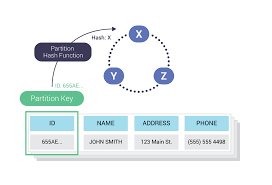
\includegraphics[width=\linewidth]{scylla_partitioning.png} % Figure image
	\caption{Sharding in Apache Cassandra} % Figure caption
	\label{scylla_ring} % Label for referencing with \ref{scylla_ring}
\end{figure}

\newpage
Bei einem Lesezugriff auf die Daten kann anhand des Wertebereichs ermittelt werden, auf welchen Nodes die Datenfiles (sog. "SSTables") gelesen werden müssen. In Apache Cassandra werden Bloom Filter eingesetzt, um zu ermitteln ob ein Datensatz in einem Datenfile vorhanden ist. Falls der Filter ein positive Ergebnis liefert und der Datensatz dennoch nicht in dem Datenfile vorhanden ist, handelt es sich um ein "false positive". Da Festplattenzugriffe auf die Disk in der Regel kostenintensiver sind als jene im Memory, wird der Bloom-Filter vollständig im Memory umgesetzt.

\section{Vor- und Nachteile}

Die folgende Tabelle beschreibt den Einsatz von Bloom-Filter gegenüber anderen Lösungsansätzen:

\begin{table}[h]
	\begin{tabularx}{\linewidth}{>{\parskip1ex}X@{\kern4\tabcolsep}>{\parskip1ex}X}
		\toprule
		\hfil\bfseries Pros
		&
		\hfil\bfseries Cons
		\\\cmidrule(r{3\tabcolsep}){1-1}\cmidrule(l{-\tabcolsep}){2-2}

		%% PROS, seperated by empty line or \par
		\lipsum[1] Anstelle der eigentlichen Daten werden nur die Hashes der Elemente gespeichert. Dadurch wird weniger Speicherkapazität benötigt.
		\par
		\lipsum[2] Das Hinzufügen und Prüfen von Elementen gehört zur Komplexitätsklasse \textit{O(k)}. Weil die verschiedenen Hashverfahren voneinander unabhängig sind, kann die Anwendung ebendieser parallelisiert werden.
		\par
		\lipsum[3] Durch die Anwendung von Hashfunktionen auf die einzelnen Werte kann der Nachteil von unregelmässig verteilten Daten verringert werden. In verteilten Datenbanken wird durch das Hashing-Verfahren eine gleichmässigere Verteilung der Daten auf den verschiedenen Datenbank-Nodes erreicht (vgl. Kapitel \ref{anwendung}).

		&
		%% CONS, seperated by empty line or \par
		\lipsum[1] Ein Bloom-Filter kann erkennen, ob ein Wort \textit{nicht} im Filter vorhanden ist - ob ein Wort allerdings mit Sicherheit im Filter vorkommt kann nicht bestimmt werden.
		\par
		\lipsum[2] Der Bloom-Filter ist einfach umzusetzen, falls Wörter nur hinzugefügt werden. Die eingangs beschriebene Funktionsweise eignet sich allerdings nicht, falls Wörter auch entfernt oder zu einem späteren Zeitpunkt geändert werden müssen.
		\par
		\lipsum[3] Wird ein Bloom-Filter erstellt, so werden die damit verbundenen Daten nicht gespeichert. Dies führt zur Einschränkung, dass nicht auf die Daten zugegriffen werden kann, da nur deren Hash-Werte im Bloom-Filter gespeichert sind.

		\\\bottomrule
	\end{tabularx}
	\caption{Gegenüberstellung Vorteile und Nachteile}
\end{table}

\section{Implementierung}
\subsection{BloomFilter-Applikation}

In der Applikation (Git-Repo: \url{https://gitlab.fhnw.ch/marco.romanutti/bloom-filter.git}) wurde ein einfacher Bloom-Filter implementiert und getestet.
Die Konfiguration kann in der Klasse \texttt{BloomFilterTest} vorgenommen werden. Die Anzahl Testwörter wird über das Attribut \texttt{wordLimit} gesetzt. Die erwartete Fehlerwahrscheinlichkeit kann direkt beim Aufruf des Konstruktors \texttt{BloomFilter(double falsePositiveProbability)} als Argument mitgegeben werden.
Um die Funktionsweise des Filters zu überprüfen, können die Tests im Verzeichnis \texttt{/src/test/} gestartet werden.

\subsection{Vergleich erwartete und effektive Fehlerwahrscheinlichkeit}

Im Verzeichnis \texttt{/src/test/} befinden sich zwei Test.
Der Test \texttt{testContainedWords} stellt sicher, dass alle Wörter des Filters auch als möglicherweise im Filter klassifitiziert werden.
Der Text \texttt{testNotContainedWords} vergleicht die erwarteten und die effektiven Fehlerwahrscheinlichkeiten.
Nach Abschluss des Tests wird eine Übersicht ausgegegeben.
Die Resultate sind in Tabelle \ref{tests} ersichtlich.

\begin{table}[h]
	\caption{Erzielte Testresultate}
	\label{tests}
	\centering
	\begin{tabular}{crrr}
		\toprule
		%\multicolumn{2}{c}{Parameter} \\
		\cmidrule(r){1-2}
		Parameter & Test(1) & Test(2) & Test(3) \\
		\midrule
		Testwörter (in Mio.) & $1.2$ & $1.2$ & $1.2$ \\
		m & $555888$ & $362329$ & $278494$ \\
		k & $7$ & $5$ & $4$ \\
		p erwartet & $0.01$ & $0.05$ & $0.1$ \\
		p effektiv & $0.0104$ & $0.0504$ & $0.1014$ \\
		\bottomrule
	\end{tabular}
\end{table}

%----------------------------------------------------------------------------------------
%	BIBLIOGRAPHY
%----------------------------------------------------------------------------------------

\begin{thebibliography}{9}
	\bibitem{wikipedia}
	Wikipedia: Bloom filter,
	\url{https://en.wikipedia.org/wiki/Bloom\_filter}

	\bibitem{scylla}
	ScyllaDB: Announcing ring architecture,
	\url{https://www.scylladb.com/2017/09/25/announcing-ring-architecture-docs/}

	\bibitem{datastax}
	Datastax: How data is distributed across a cluster,
	\url{https://docs.datastax.com/en/cassandra/3.0/cassandra/architecture/archDataDistributeDistribute.html}
\end{thebibliography}
%----------------------------------------------------------------------------------------

\end{document}
